\section{Deletion}
In a mature VM cluster, snapshot deletions are as frequent as snapshot creations.
Our system adopts lazy delete strategy so that all snapshot deletions are scheduled
in the backup time window at midnight. 
Therefore, snapshot deletions must be fast enough to fit in time window and
efficient enough to satisfy our resource constraints.
However, there is no simple solution can achieve these goals with high reliability.
In Aliyun's cloud, we use a {\em fuzzy deletion} method to trade deletion accuracy for
speed and resource usage. This method tolerates a tiny percentage of storage leakage
to make the deletion operation faster and efficient by an order of magnitude,
yet we still adopt an slow but accurate deletion method to fix such leakage in the long-term.
Our hybrid deletion strategy, using fuzzy deletion regularly and accurate deletion periodically,
accomplishs our speed, resource usage and relibility goals very well.

% \subsection{Challenges}
% Contrary to a traditional backup system, a dedupe system shares data among files by default. 
% Reference management is necessary to keep track of chunk usage and reclaim freed space. 
% In addition to scalability and speed, reliability is another challenge for reference management. 
% If a chunk gets freed while it is still referenced by snapshots, data loss occurs and files cannot be restored. 
% On the other hand, if a chunk is referenced when it is actually no longer in use, it causes storage leakage.

% Reference counting, while being simple, suffers from low reliability especially in our distributed environment, 
% because it is vulnerable to lost or repeated updates: when errors occur some chunks maybe updated and some may not. 
% Complicated transaction rollback logic is required to make reference counts consistent. Moreover, 
% there is almost no way to verify if the reference count is correct or not in a large dynamic system. 
% In real deployments, where data integrity and recoverability directly affect product reputation, simple reference counting is unsatisfactory.

% Mark-and-sweep is generally a better solution. During the mark phase, all snapshot recipes are traversed so as to mark the used chunks. 
% In the sweep phase all chunks are swept and unmarked chunks are reclaimed. 
% This approach is very resilient to errors: at any time the process can simply be restarted with no negative side effects. 
% Scalability, however, is an issue. {\em needs to explain its resource usage}


\subsection{Approximate Deletion}
\begin{figure}[htbp]
  \centering
  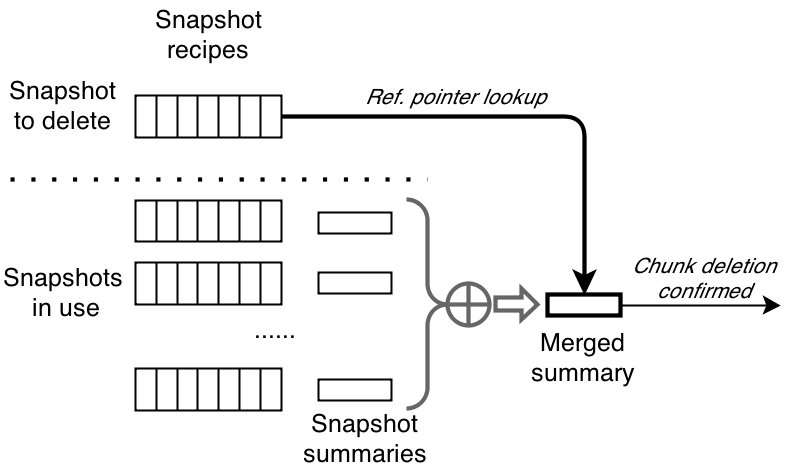
\epsfig{file=images/deletion.png, width=3.5in}
  \caption{Approximate deletion}
  \label{fig:deletion_flow}
\end{figure}

We design approximate deletion to fast identify unused data in the append store.
Instead of scanning the whold append store, it uses a Bloom filter to check 
if a data are still referenced by living snapshots. However, there is a small false-positive probility which
would indetify unused data as in use, i.e., storage leakage.
The following steps would take place during an approximate deletion:

\begin{enumerate}
\item {\bf Creating Bloom filter} Scan all the living snapshot recipess and their segment recipes,
for every reference pointing to append store, add it to the Bloom filter.
\item {\bf Check existance} For every data reference in the deleted snapshot recipe and its segment recipes,
check the existance of that data reference in Bloom filter. If not found, it is safe to delete that piece of data from append store
because no living snapshots has referenced it.
\end{enumerate}

The overall time of running a approximate deletion for one snapshot deletion would be scanning
all the living snapshots and deleted snapshots, since operations on the in-memory Bloom filter can be done in
parallel and is much faster than loading recipes from DFS:
\begin{equation}
T = (N_{SS} + 1) * T_{scan\_recipes}
\end{equation}
 
Using the example and analysis in previous section, this approximate deletion can be done in 5 minutes. 
Memory usage of the Bloom filter depends on its false-positive probility $P_{bl}$,
when set $P_{bl}$ to 0.01, the memory footprint of approximate deletion is about 15 MB.

The design goal of approximate deletion is to reduce the frequency of running accurate deletion.
For one VM's snapshots, let $D_{leakage}$ be the amount of storage leakage, $D_{del}$ be the average amount of data
to be deleted in one snapshot deletion, 
then we have:
\begin{equation}
D_{leakage} = N_{approximate} * P_{bl} * D_{del}
\end{equation}
where $N_{approximate}$ is the number of runs of approximate deletion. 
An accurate deletion is triggered to fix the storage leakage
when $D_{leakage}/D_{del}$ is accmulated to exceed certain threshold $T$:
\begin{equation}
D_{leakage} / D_{del} = N_{approximate} * P_{bl} > T \Rightarrow N_{approximate} > T/P_{bl}
\end{equation}
Therefore, when $P_{bl} = 0.01$ and $T=1$, 
there would be a run of accurate deletion for every $T/P_{bl} = 100$ runs of approximate deletion.
On a machine that hosts 20 VMs and each VM deletes snapshot daily, there would be less than
one accurate deletion scheduled per day.

\subsection{Accurate Deletion}
Our accurate deletion uses mark-and-sweep to find all the unused chunks in a VM's append store.
The following steps would take place during an accurate deletion:

\begin{enumerate}
\item Scan all the containers. For each container, extract full list of existing data references and allocate a bitmap. 
(Notice this list is self sorted.)
\item Scan all the snapshot recipes and segment recipes. For every data reference pointing to append store,
find it in the above lists and mark the corresponding position in bitmaps.
\item Scan the bitmaps, for every bit that are not marked, tell append store the corresponding data reference can be deleted.
\end{enumerate}

Although accurate deletion guarantees reliability and correctness, its speed and resource usage are big problems to our VM cloud.
Let $T_{scan\_AS}$ be the time to scan the VM's append store, $T_{scan\_recipes}$ be the time to scan one snapshot recipe
and its segment recipes, $T_{mark}$ be the time of finding a data reference in the list and mark bitmap, 
$N_{SS}$ be the number of snapshots and $N_c$ be the number of chunks in one snapshot.
The overall time of running an accurate deletion for one VM is:
\begin{equation}
T = T_{scan\_AS} + N_{SS} * T_{scan\_recipes} + N_{SS} * N_c * T_{mark}
\end{equation}

For a virtual disk that has 10 snapshots, 50 GB of data in the append store, $T_{scan\_AS}$ would have cost half an hour already.
In addition, scanning recipes of 10 snapshots cost another 5 minutes.
Furthermore, maintaining the full lists of data references and bitmaps costs about 100 MB of memory. Having tens of VMs
co-lived in one physical machine and deleting snapshot on a daily basis, 
it's infeasible to run accurate deletion as frequent as snapshot deletions.

\subsection{Discussion}
